% Created by tikzDevice version 0.12.3.1 on 2022-05-02 14:17:35
% !TEX encoding = UTF-8 Unicode
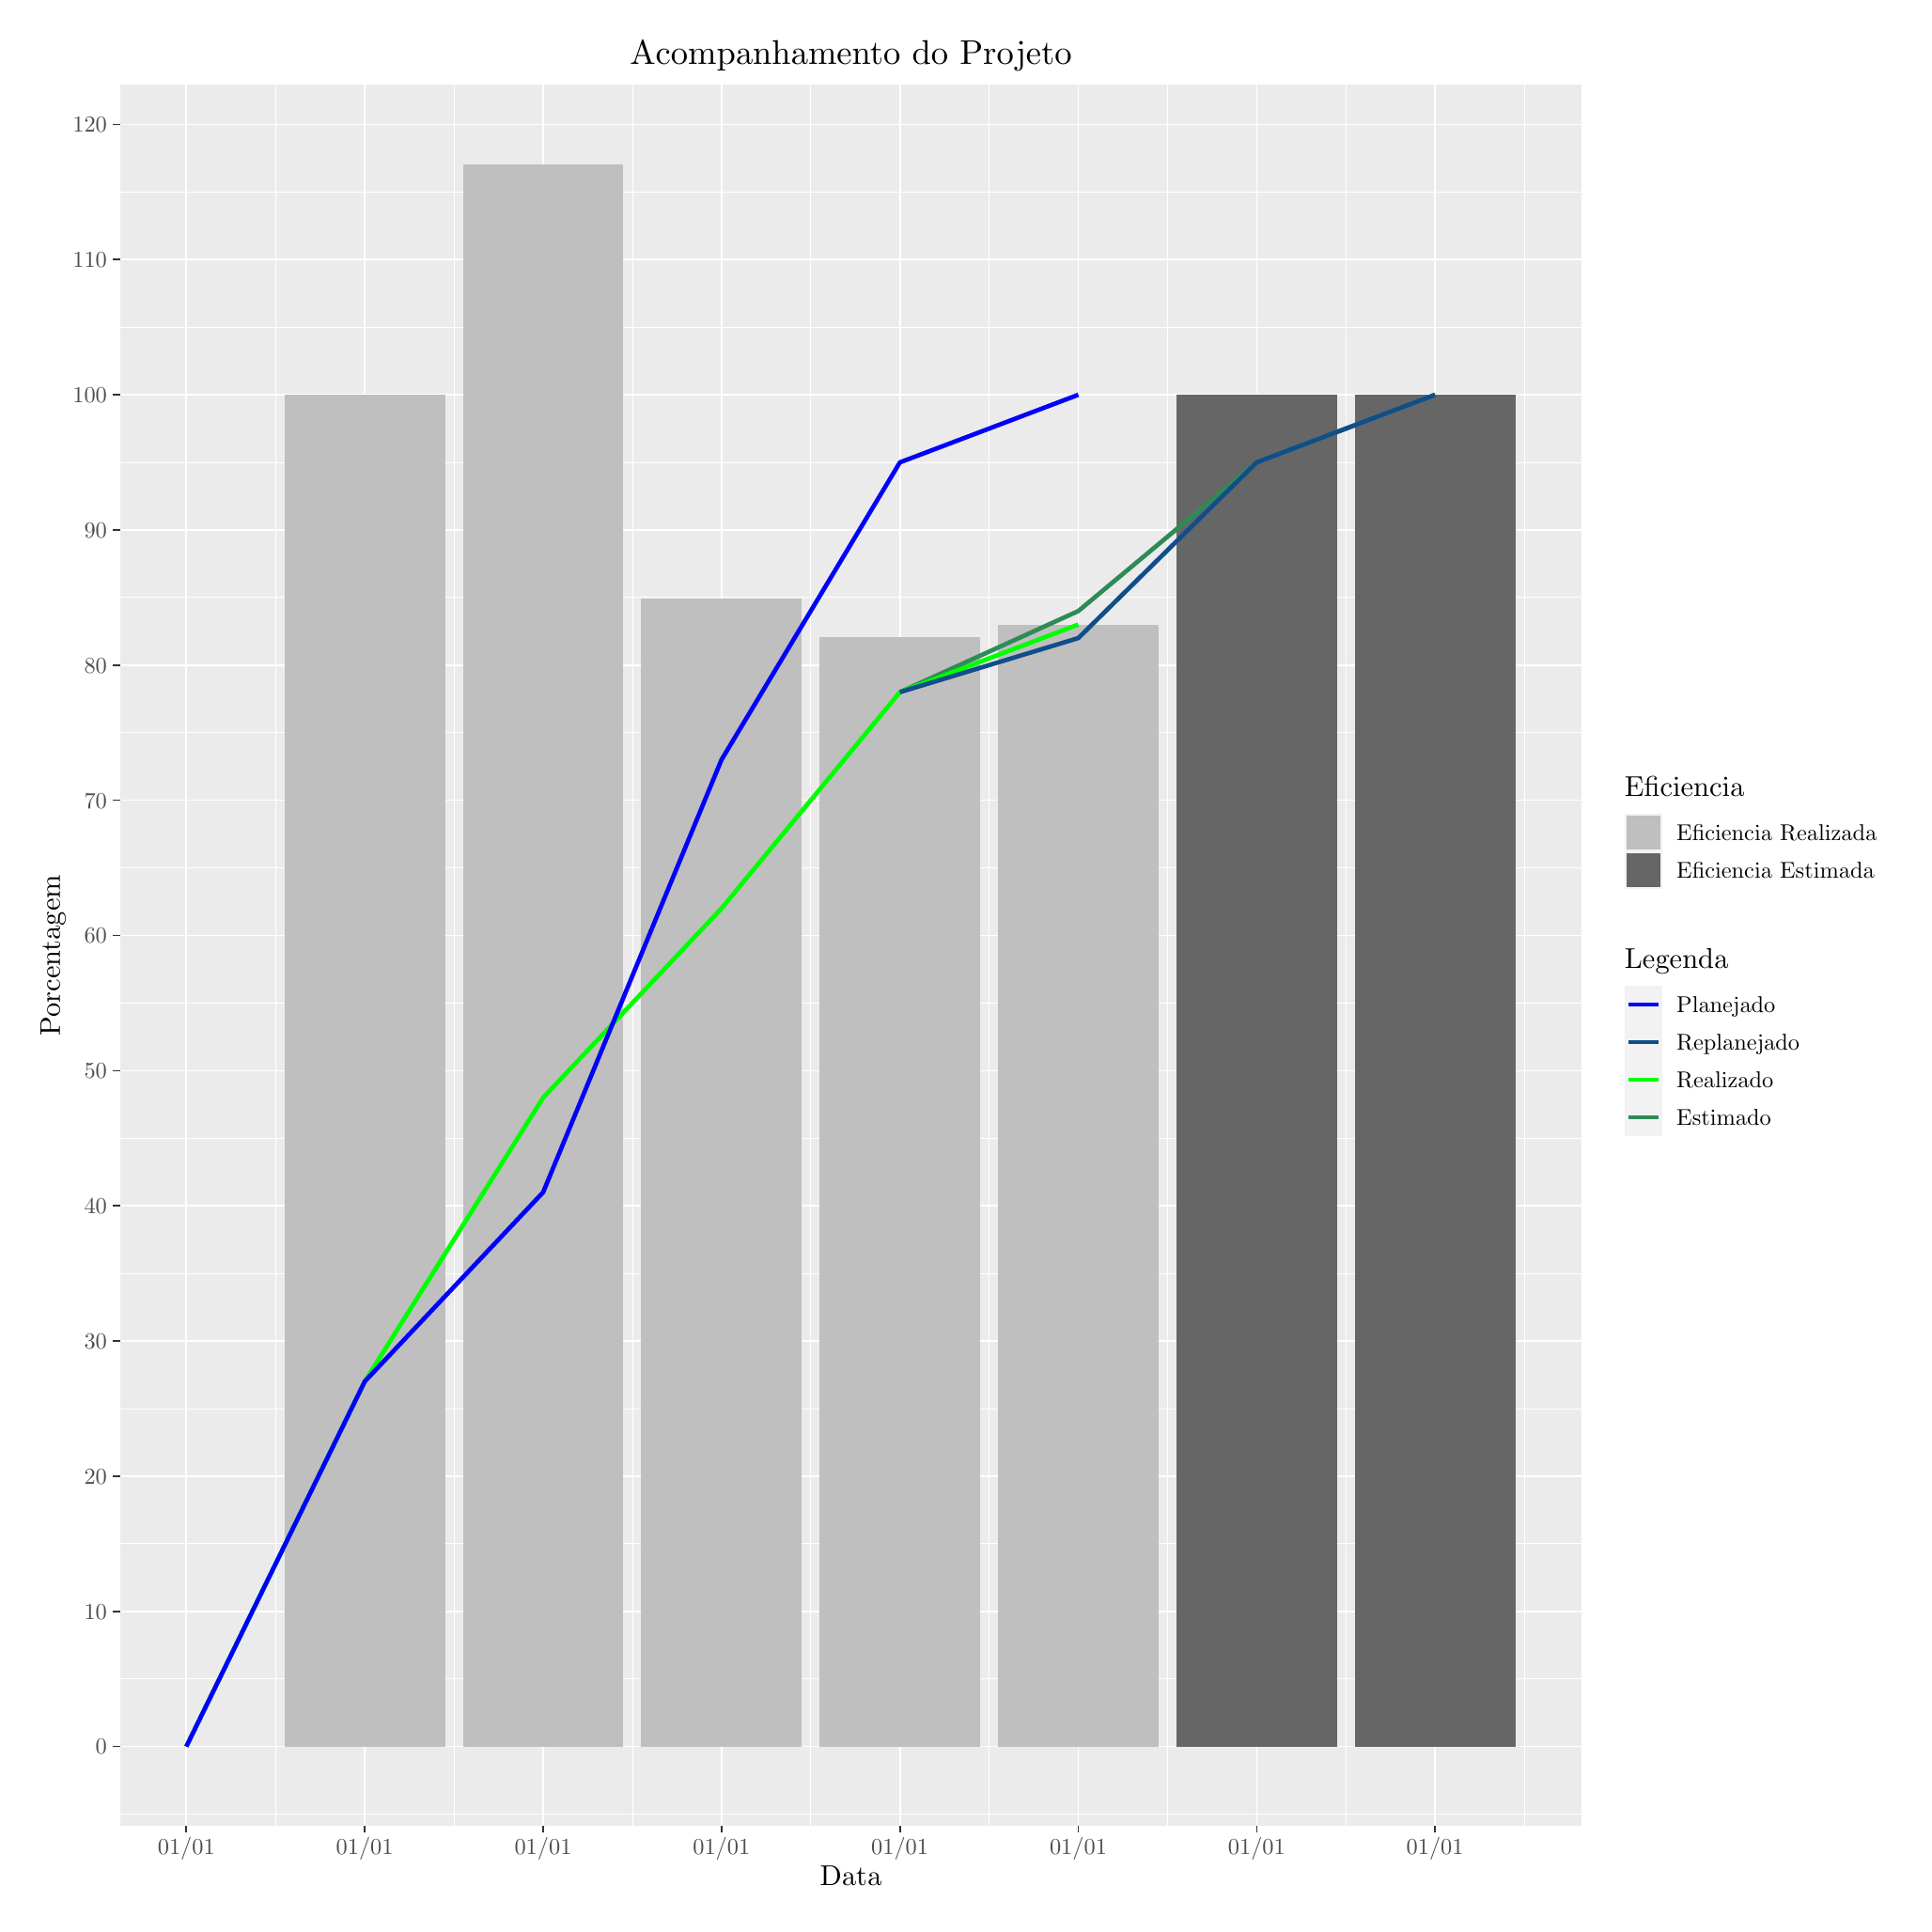
\begin{tikzpicture}[x=1pt,y=1pt]
\definecolor{fillColor}{RGB}{255,255,255}
\path[use as bounding box,fill=fillColor,fill opacity=0.00] (0,0) rectangle (722.70,722.70);
\begin{scope}
\path[clip] (  0.00,  0.00) rectangle (722.70,722.70);
\definecolor{drawColor}{RGB}{255,255,255}
\definecolor{fillColor}{RGB}{255,255,255}

\path[draw=drawColor,line width= 0.6pt,line join=round,line cap=round,fill=fillColor] (  0.00,  0.00) rectangle (722.70,722.70);
\end{scope}
\begin{scope}
\path[clip] ( 36.11, 30.69) rectangle (598.26,700.04);
\definecolor{fillColor}{gray}{0.92}

\path[fill=fillColor] ( 36.11, 30.69) rectangle (598.26,700.04);
\definecolor{drawColor}{RGB}{255,255,255}

\path[draw=drawColor,line width= 0.3pt,line join=round] ( 36.11, 35.12) --
	(598.26, 35.12);

\path[draw=drawColor,line width= 0.3pt,line join=round] ( 36.11, 87.10) --
	(598.26, 87.10);

\path[draw=drawColor,line width= 0.3pt,line join=round] ( 36.11,139.08) --
	(598.26,139.08);

\path[draw=drawColor,line width= 0.3pt,line join=round] ( 36.11,191.05) --
	(598.26,191.05);

\path[draw=drawColor,line width= 0.3pt,line join=round] ( 36.11,243.03) --
	(598.26,243.03);

\path[draw=drawColor,line width= 0.3pt,line join=round] ( 36.11,295.01) --
	(598.26,295.01);

\path[draw=drawColor,line width= 0.3pt,line join=round] ( 36.11,346.98) --
	(598.26,346.98);

\path[draw=drawColor,line width= 0.3pt,line join=round] ( 36.11,398.96) --
	(598.26,398.96);

\path[draw=drawColor,line width= 0.3pt,line join=round] ( 36.11,450.94) --
	(598.26,450.94);

\path[draw=drawColor,line width= 0.3pt,line join=round] ( 36.11,502.91) --
	(598.26,502.91);

\path[draw=drawColor,line width= 0.3pt,line join=round] ( 36.11,554.89) --
	(598.26,554.89);

\path[draw=drawColor,line width= 0.3pt,line join=round] ( 36.11,606.87) --
	(598.26,606.87);

\path[draw=drawColor,line width= 0.3pt,line join=round] ( 36.11,658.84) --
	(598.26,658.84);

\path[draw=drawColor,line width= 0.3pt,line join=round] ( 95.96, 30.69) --
	( 95.96,700.04);

\path[draw=drawColor,line width= 0.3pt,line join=round] (164.56, 30.69) --
	(164.56,700.04);

\path[draw=drawColor,line width= 0.3pt,line join=round] (233.16, 30.69) --
	(233.16,700.04);

\path[draw=drawColor,line width= 0.3pt,line join=round] (301.75, 30.69) --
	(301.75,700.04);

\path[draw=drawColor,line width= 0.3pt,line join=round] (370.35, 30.69) --
	(370.35,700.04);

\path[draw=drawColor,line width= 0.3pt,line join=round] (438.95, 30.69) --
	(438.95,700.04);

\path[draw=drawColor,line width= 0.3pt,line join=round] (507.54, 30.69) --
	(507.54,700.04);

\path[draw=drawColor,line width= 0.3pt,line join=round] (576.14, 30.69) --
	(576.14,700.04);

\path[draw=drawColor,line width= 0.6pt,line join=round] ( 36.11, 61.11) --
	(598.26, 61.11);

\path[draw=drawColor,line width= 0.6pt,line join=round] ( 36.11,113.09) --
	(598.26,113.09);

\path[draw=drawColor,line width= 0.6pt,line join=round] ( 36.11,165.06) --
	(598.26,165.06);

\path[draw=drawColor,line width= 0.6pt,line join=round] ( 36.11,217.04) --
	(598.26,217.04);

\path[draw=drawColor,line width= 0.6pt,line join=round] ( 36.11,269.02) --
	(598.26,269.02);

\path[draw=drawColor,line width= 0.6pt,line join=round] ( 36.11,320.99) --
	(598.26,320.99);

\path[draw=drawColor,line width= 0.6pt,line join=round] ( 36.11,372.97) --
	(598.26,372.97);

\path[draw=drawColor,line width= 0.6pt,line join=round] ( 36.11,424.95) --
	(598.26,424.95);

\path[draw=drawColor,line width= 0.6pt,line join=round] ( 36.11,476.92) --
	(598.26,476.92);

\path[draw=drawColor,line width= 0.6pt,line join=round] ( 36.11,528.90) --
	(598.26,528.90);

\path[draw=drawColor,line width= 0.6pt,line join=round] ( 36.11,580.88) --
	(598.26,580.88);

\path[draw=drawColor,line width= 0.6pt,line join=round] ( 36.11,632.85) --
	(598.26,632.85);

\path[draw=drawColor,line width= 0.6pt,line join=round] ( 36.11,684.83) --
	(598.26,684.83);

\path[draw=drawColor,line width= 0.6pt,line join=round] ( 61.66, 30.69) --
	( 61.66,700.04);

\path[draw=drawColor,line width= 0.6pt,line join=round] (130.26, 30.69) --
	(130.26,700.04);

\path[draw=drawColor,line width= 0.6pt,line join=round] (198.86, 30.69) --
	(198.86,700.04);

\path[draw=drawColor,line width= 0.6pt,line join=round] (267.45, 30.69) --
	(267.45,700.04);

\path[draw=drawColor,line width= 0.6pt,line join=round] (336.05, 30.69) --
	(336.05,700.04);

\path[draw=drawColor,line width= 0.6pt,line join=round] (404.65, 30.69) --
	(404.65,700.04);

\path[draw=drawColor,line width= 0.6pt,line join=round] (473.25, 30.69) --
	(473.25,700.04);

\path[draw=drawColor,line width= 0.6pt,line join=round] (541.84, 30.69) --
	(541.84,700.04);
\definecolor{fillColor}{gray}{0.75}

\path[fill=fillColor] ( 99.39, 61.11) rectangle (161.13,580.88);

\path[fill=fillColor] (167.99, 61.11) rectangle (229.73,669.62);

\path[fill=fillColor] (236.59, 61.11) rectangle (298.32,502.56);

\path[fill=fillColor] (305.18, 61.11) rectangle (366.92,487.87);

\path[fill=fillColor] (373.78, 61.11) rectangle (435.52,492.52);
\definecolor{fillColor}{gray}{0.40}

\path[fill=fillColor] (442.38, 61.11) rectangle (504.11,580.88);

\path[fill=fillColor] (510.97, 61.11) rectangle (572.71,580.88);
\definecolor{drawColor}{RGB}{46,139,87}

\path[draw=drawColor,line width= 1.7pt,line join=round] (336.05,466.53) --
	(404.65,497.71) --
	(473.25,554.89) --
	(541.84,580.88);
\definecolor{drawColor}{RGB}{0,255,0}

\path[draw=drawColor,line width= 1.7pt,line join=round] ( 61.66, 61.11) --
	(130.26,201.45) --
	(198.86,310.60) --
	(267.45,383.37) --
	(336.05,466.53) --
	(404.65,492.52);
\definecolor{drawColor}{RGB}{0,0,255}

\path[draw=drawColor,line width= 1.7pt,line join=round] ( 61.66, 61.11) --
	(130.26,201.45) --
	(198.86,274.22) --
	(267.45,440.54) --
	(336.05,554.89) --
	(404.65,580.88);
\definecolor{drawColor}{RGB}{16,78,139}

\path[draw=drawColor,line width= 1.7pt,line join=round] (336.05,466.53) --
	(404.65,487.32) --
	(473.25,554.89) --
	(541.84,580.88);
\end{scope}
\begin{scope}
\path[clip] (  0.00,  0.00) rectangle (722.70,722.70);
\definecolor{drawColor}{gray}{0.30}

\node[text=drawColor,anchor=base east,inner sep=0pt, outer sep=0pt, scale=  0.88] at ( 31.16, 58.08) {0};

\node[text=drawColor,anchor=base east,inner sep=0pt, outer sep=0pt, scale=  0.88] at ( 31.16,110.06) {10};

\node[text=drawColor,anchor=base east,inner sep=0pt, outer sep=0pt, scale=  0.88] at ( 31.16,162.03) {20};

\node[text=drawColor,anchor=base east,inner sep=0pt, outer sep=0pt, scale=  0.88] at ( 31.16,214.01) {30};

\node[text=drawColor,anchor=base east,inner sep=0pt, outer sep=0pt, scale=  0.88] at ( 31.16,265.99) {40};

\node[text=drawColor,anchor=base east,inner sep=0pt, outer sep=0pt, scale=  0.88] at ( 31.16,317.96) {50};

\node[text=drawColor,anchor=base east,inner sep=0pt, outer sep=0pt, scale=  0.88] at ( 31.16,369.94) {60};

\node[text=drawColor,anchor=base east,inner sep=0pt, outer sep=0pt, scale=  0.88] at ( 31.16,421.92) {70};

\node[text=drawColor,anchor=base east,inner sep=0pt, outer sep=0pt, scale=  0.88] at ( 31.16,473.89) {80};

\node[text=drawColor,anchor=base east,inner sep=0pt, outer sep=0pt, scale=  0.88] at ( 31.16,525.87) {90};

\node[text=drawColor,anchor=base east,inner sep=0pt, outer sep=0pt, scale=  0.88] at ( 31.16,577.85) {100};

\node[text=drawColor,anchor=base east,inner sep=0pt, outer sep=0pt, scale=  0.88] at ( 31.16,629.82) {110};

\node[text=drawColor,anchor=base east,inner sep=0pt, outer sep=0pt, scale=  0.88] at ( 31.16,681.80) {120};
\end{scope}
\begin{scope}
\path[clip] (  0.00,  0.00) rectangle (722.70,722.70);
\definecolor{drawColor}{gray}{0.20}

\path[draw=drawColor,line width= 0.6pt,line join=round] ( 33.36, 61.11) --
	( 36.11, 61.11);

\path[draw=drawColor,line width= 0.6pt,line join=round] ( 33.36,113.09) --
	( 36.11,113.09);

\path[draw=drawColor,line width= 0.6pt,line join=round] ( 33.36,165.06) --
	( 36.11,165.06);

\path[draw=drawColor,line width= 0.6pt,line join=round] ( 33.36,217.04) --
	( 36.11,217.04);

\path[draw=drawColor,line width= 0.6pt,line join=round] ( 33.36,269.02) --
	( 36.11,269.02);

\path[draw=drawColor,line width= 0.6pt,line join=round] ( 33.36,320.99) --
	( 36.11,320.99);

\path[draw=drawColor,line width= 0.6pt,line join=round] ( 33.36,372.97) --
	( 36.11,372.97);

\path[draw=drawColor,line width= 0.6pt,line join=round] ( 33.36,424.95) --
	( 36.11,424.95);

\path[draw=drawColor,line width= 0.6pt,line join=round] ( 33.36,476.92) --
	( 36.11,476.92);

\path[draw=drawColor,line width= 0.6pt,line join=round] ( 33.36,528.90) --
	( 36.11,528.90);

\path[draw=drawColor,line width= 0.6pt,line join=round] ( 33.36,580.88) --
	( 36.11,580.88);

\path[draw=drawColor,line width= 0.6pt,line join=round] ( 33.36,632.85) --
	( 36.11,632.85);

\path[draw=drawColor,line width= 0.6pt,line join=round] ( 33.36,684.83) --
	( 36.11,684.83);
\end{scope}
\begin{scope}
\path[clip] (  0.00,  0.00) rectangle (722.70,722.70);
\definecolor{drawColor}{gray}{0.20}

\path[draw=drawColor,line width= 0.6pt,line join=round] ( 61.66, 27.94) --
	( 61.66, 30.69);

\path[draw=drawColor,line width= 0.6pt,line join=round] (130.26, 27.94) --
	(130.26, 30.69);

\path[draw=drawColor,line width= 0.6pt,line join=round] (198.86, 27.94) --
	(198.86, 30.69);

\path[draw=drawColor,line width= 0.6pt,line join=round] (267.45, 27.94) --
	(267.45, 30.69);

\path[draw=drawColor,line width= 0.6pt,line join=round] (336.05, 27.94) --
	(336.05, 30.69);

\path[draw=drawColor,line width= 0.6pt,line join=round] (404.65, 27.94) --
	(404.65, 30.69);

\path[draw=drawColor,line width= 0.6pt,line join=round] (473.25, 27.94) --
	(473.25, 30.69);

\path[draw=drawColor,line width= 0.6pt,line join=round] (541.84, 27.94) --
	(541.84, 30.69);
\end{scope}
\begin{scope}
\path[clip] (  0.00,  0.00) rectangle (722.70,722.70);
\definecolor{drawColor}{gray}{0.30}

\node[text=drawColor,anchor=base,inner sep=0pt, outer sep=0pt, scale=  0.88] at ( 61.66, 19.68) {01/01};

\node[text=drawColor,anchor=base,inner sep=0pt, outer sep=0pt, scale=  0.88] at (130.26, 19.68) {01/01};

\node[text=drawColor,anchor=base,inner sep=0pt, outer sep=0pt, scale=  0.88] at (198.86, 19.68) {01/01};

\node[text=drawColor,anchor=base,inner sep=0pt, outer sep=0pt, scale=  0.88] at (267.45, 19.68) {01/01};

\node[text=drawColor,anchor=base,inner sep=0pt, outer sep=0pt, scale=  0.88] at (336.05, 19.68) {01/01};

\node[text=drawColor,anchor=base,inner sep=0pt, outer sep=0pt, scale=  0.88] at (404.65, 19.68) {01/01};

\node[text=drawColor,anchor=base,inner sep=0pt, outer sep=0pt, scale=  0.88] at (473.25, 19.68) {01/01};

\node[text=drawColor,anchor=base,inner sep=0pt, outer sep=0pt, scale=  0.88] at (541.84, 19.68) {01/01};
\end{scope}
\begin{scope}
\path[clip] (  0.00,  0.00) rectangle (722.70,722.70);
\definecolor{drawColor}{RGB}{0,0,0}

\node[text=drawColor,anchor=base,inner sep=0pt, outer sep=0pt, scale=  1.10] at (317.19,  7.64) {Data};
\end{scope}
\begin{scope}
\path[clip] (  0.00,  0.00) rectangle (722.70,722.70);
\definecolor{drawColor}{RGB}{0,0,0}

\node[text=drawColor,rotate= 90.00,anchor=base,inner sep=0pt, outer sep=0pt, scale=  1.10] at ( 13.08,365.36) {Porcentagem};
\end{scope}
\begin{scope}
\path[clip] (  0.00,  0.00) rectangle (722.70,722.70);
\definecolor{fillColor}{RGB}{255,255,255}

\path[fill=fillColor] (609.26,385.32) rectangle (717.20,440.44);
\end{scope}
\begin{scope}
\path[clip] (  0.00,  0.00) rectangle (722.70,722.70);
\definecolor{drawColor}{RGB}{0,0,0}

\node[text=drawColor,anchor=base west,inner sep=0pt, outer sep=0pt, scale=  1.10] at (614.76,426.30) {Eficiencia};
\end{scope}
\begin{scope}
\path[clip] (  0.00,  0.00) rectangle (722.70,722.70);
\definecolor{fillColor}{gray}{0.95}

\path[fill=fillColor] (614.76,405.27) rectangle (629.22,419.73);
\end{scope}
\begin{scope}
\path[clip] (  0.00,  0.00) rectangle (722.70,722.70);
\definecolor{fillColor}{gray}{0.75}

\path[fill=fillColor] (615.48,405.98) rectangle (628.51,419.01);
\end{scope}
\begin{scope}
\path[clip] (  0.00,  0.00) rectangle (722.70,722.70);
\definecolor{fillColor}{gray}{0.75}

\path[fill=fillColor] (615.48,405.98) rectangle (628.51,419.01);
\end{scope}
\begin{scope}
\path[clip] (  0.00,  0.00) rectangle (722.70,722.70);
\definecolor{fillColor}{gray}{0.95}

\path[fill=fillColor] (614.76,390.82) rectangle (629.22,405.27);
\end{scope}
\begin{scope}
\path[clip] (  0.00,  0.00) rectangle (722.70,722.70);
\definecolor{fillColor}{gray}{0.40}

\path[fill=fillColor] (615.48,391.53) rectangle (628.51,404.56);
\end{scope}
\begin{scope}
\path[clip] (  0.00,  0.00) rectangle (722.70,722.70);
\definecolor{fillColor}{gray}{0.40}

\path[fill=fillColor] (615.48,391.53) rectangle (628.51,404.56);
\end{scope}
\begin{scope}
\path[clip] (  0.00,  0.00) rectangle (722.70,722.70);
\definecolor{drawColor}{RGB}{0,0,0}

\node[text=drawColor,anchor=base west,inner sep=0pt, outer sep=0pt, scale=  0.88] at (634.72,409.47) {Eficiencia Realizada};
\end{scope}
\begin{scope}
\path[clip] (  0.00,  0.00) rectangle (722.70,722.70);
\definecolor{drawColor}{RGB}{0,0,0}

\node[text=drawColor,anchor=base west,inner sep=0pt, outer sep=0pt, scale=  0.88] at (634.72,395.01) {Eficiencia Estimada};
\end{scope}
\begin{scope}
\path[clip] (  0.00,  0.00) rectangle (722.70,722.70);
\definecolor{fillColor}{RGB}{255,255,255}

\path[fill=fillColor] (609.26,290.29) rectangle (687.51,374.32);
\end{scope}
\begin{scope}
\path[clip] (  0.00,  0.00) rectangle (722.70,722.70);
\definecolor{drawColor}{RGB}{0,0,0}

\node[text=drawColor,anchor=base west,inner sep=0pt, outer sep=0pt, scale=  1.10] at (614.76,360.17) {Legenda};
\end{scope}
\begin{scope}
\path[clip] (  0.00,  0.00) rectangle (722.70,722.70);
\definecolor{fillColor}{gray}{0.95}

\path[fill=fillColor] (614.76,339.15) rectangle (629.22,353.60);
\end{scope}
\begin{scope}
\path[clip] (  0.00,  0.00) rectangle (722.70,722.70);
\definecolor{drawColor}{RGB}{0,0,255}

\path[draw=drawColor,line width= 1.7pt,line join=round] (616.21,346.38) -- (627.77,346.38);
\end{scope}
\begin{scope}
\path[clip] (  0.00,  0.00) rectangle (722.70,722.70);
\definecolor{drawColor}{RGB}{0,0,255}

\path[draw=drawColor,line width= 1.7pt,line join=round] (616.21,346.38) -- (627.77,346.38);
\end{scope}
\begin{scope}
\path[clip] (  0.00,  0.00) rectangle (722.70,722.70);
\definecolor{drawColor}{RGB}{0,0,255}

\path[draw=drawColor,line width= 1.7pt,line join=round] (616.21,346.38) -- (627.77,346.38);
\end{scope}
\begin{scope}
\path[clip] (  0.00,  0.00) rectangle (722.70,722.70);
\definecolor{drawColor}{RGB}{0,0,255}

\path[draw=drawColor,line width= 1.7pt,line join=round] (616.21,346.38) -- (627.77,346.38);
\end{scope}
\begin{scope}
\path[clip] (  0.00,  0.00) rectangle (722.70,722.70);
\definecolor{fillColor}{gray}{0.95}

\path[fill=fillColor] (614.76,324.70) rectangle (629.22,339.15);
\end{scope}
\begin{scope}
\path[clip] (  0.00,  0.00) rectangle (722.70,722.70);
\definecolor{drawColor}{RGB}{16,78,139}

\path[draw=drawColor,line width= 1.7pt,line join=round] (616.21,331.92) -- (627.77,331.92);
\end{scope}
\begin{scope}
\path[clip] (  0.00,  0.00) rectangle (722.70,722.70);
\definecolor{drawColor}{RGB}{16,78,139}

\path[draw=drawColor,line width= 1.7pt,line join=round] (616.21,331.92) -- (627.77,331.92);
\end{scope}
\begin{scope}
\path[clip] (  0.00,  0.00) rectangle (722.70,722.70);
\definecolor{drawColor}{RGB}{16,78,139}

\path[draw=drawColor,line width= 1.7pt,line join=round] (616.21,331.92) -- (627.77,331.92);
\end{scope}
\begin{scope}
\path[clip] (  0.00,  0.00) rectangle (722.70,722.70);
\definecolor{drawColor}{RGB}{16,78,139}

\path[draw=drawColor,line width= 1.7pt,line join=round] (616.21,331.92) -- (627.77,331.92);
\end{scope}
\begin{scope}
\path[clip] (  0.00,  0.00) rectangle (722.70,722.70);
\definecolor{fillColor}{gray}{0.95}

\path[fill=fillColor] (614.76,310.24) rectangle (629.22,324.70);
\end{scope}
\begin{scope}
\path[clip] (  0.00,  0.00) rectangle (722.70,722.70);
\definecolor{drawColor}{RGB}{0,255,0}

\path[draw=drawColor,line width= 1.7pt,line join=round] (616.21,317.47) -- (627.77,317.47);
\end{scope}
\begin{scope}
\path[clip] (  0.00,  0.00) rectangle (722.70,722.70);
\definecolor{drawColor}{RGB}{0,255,0}

\path[draw=drawColor,line width= 1.7pt,line join=round] (616.21,317.47) -- (627.77,317.47);
\end{scope}
\begin{scope}
\path[clip] (  0.00,  0.00) rectangle (722.70,722.70);
\definecolor{drawColor}{RGB}{0,255,0}

\path[draw=drawColor,line width= 1.7pt,line join=round] (616.21,317.47) -- (627.77,317.47);
\end{scope}
\begin{scope}
\path[clip] (  0.00,  0.00) rectangle (722.70,722.70);
\definecolor{drawColor}{RGB}{0,255,0}

\path[draw=drawColor,line width= 1.7pt,line join=round] (616.21,317.47) -- (627.77,317.47);
\end{scope}
\begin{scope}
\path[clip] (  0.00,  0.00) rectangle (722.70,722.70);
\definecolor{fillColor}{gray}{0.95}

\path[fill=fillColor] (614.76,295.79) rectangle (629.22,310.24);
\end{scope}
\begin{scope}
\path[clip] (  0.00,  0.00) rectangle (722.70,722.70);
\definecolor{drawColor}{RGB}{46,139,87}

\path[draw=drawColor,line width= 1.7pt,line join=round] (616.21,303.01) -- (627.77,303.01);
\end{scope}
\begin{scope}
\path[clip] (  0.00,  0.00) rectangle (722.70,722.70);
\definecolor{drawColor}{RGB}{46,139,87}

\path[draw=drawColor,line width= 1.7pt,line join=round] (616.21,303.01) -- (627.77,303.01);
\end{scope}
\begin{scope}
\path[clip] (  0.00,  0.00) rectangle (722.70,722.70);
\definecolor{drawColor}{RGB}{46,139,87}

\path[draw=drawColor,line width= 1.7pt,line join=round] (616.21,303.01) -- (627.77,303.01);
\end{scope}
\begin{scope}
\path[clip] (  0.00,  0.00) rectangle (722.70,722.70);
\definecolor{drawColor}{RGB}{46,139,87}

\path[draw=drawColor,line width= 1.7pt,line join=round] (616.21,303.01) -- (627.77,303.01);
\end{scope}
\begin{scope}
\path[clip] (  0.00,  0.00) rectangle (722.70,722.70);
\definecolor{drawColor}{RGB}{0,0,0}

\node[text=drawColor,anchor=base west,inner sep=0pt, outer sep=0pt, scale=  0.88] at (634.72,343.35) {Planejado};
\end{scope}
\begin{scope}
\path[clip] (  0.00,  0.00) rectangle (722.70,722.70);
\definecolor{drawColor}{RGB}{0,0,0}

\node[text=drawColor,anchor=base west,inner sep=0pt, outer sep=0pt, scale=  0.88] at (634.72,328.89) {Replanejado};
\end{scope}
\begin{scope}
\path[clip] (  0.00,  0.00) rectangle (722.70,722.70);
\definecolor{drawColor}{RGB}{0,0,0}

\node[text=drawColor,anchor=base west,inner sep=0pt, outer sep=0pt, scale=  0.88] at (634.72,314.44) {Realizado};
\end{scope}
\begin{scope}
\path[clip] (  0.00,  0.00) rectangle (722.70,722.70);
\definecolor{drawColor}{RGB}{0,0,0}

\node[text=drawColor,anchor=base west,inner sep=0pt, outer sep=0pt, scale=  0.88] at (634.72,299.98) {Estimado};
\end{scope}
\begin{scope}
\path[clip] (  0.00,  0.00) rectangle (722.70,722.70);
\definecolor{drawColor}{RGB}{0,0,0}

\node[text=drawColor,anchor=base,inner sep=0pt, outer sep=0pt, scale=  1.32] at (317.19,708.11) {Acompanhamento do Projeto};
\end{scope}
\end{tikzpicture}
